\chapter{Abbildungen}
\label{sec:tikz}

Bei wissenschaftlichen Arbeiten sollten aussagekräftige Bildunterschriften angefertigt werden. Abbildungen sind meist nicht als selbsterklärend zu verstehen. Daher müssen zusätzliche Beschreibungen in die Bildunterschrift eingefügt werden, die es dem Leser möglichst erlauben, nur durch die Abbildung und dessen Beschreibung die im Fließtext erläuterten Zusammenhänge zusammengefasst zu verstehen oder mindestens die Bedeutung der Abbildung für Teile des Fließtextes klar einordnen zu können.

Zur Erstellung von aufschlussreichen Abbildungen siehe auch das \verb!Graphic-design-cheat-sheet.pdf!

\section{Einfügen von Bildern}
\label{sec:graf}

\subsection{Einfaches Bild}

\begin{figure}[H]
  \centering  
  	
\includegraphics[scale=0.5]{ILEK-logo.jpg}
  \caption{ILEK Logo}
  \label{fig:05_starwars}
\end{figure}

\subsection{Gruppierung von Bildern}

\begin{figure}[H]
	\centering
	\begin{subfigure}[b]{0.3\textwidth}
		\centering
		
\includegraphics[width=\textwidth]{ILEK-logo.jpg}
		\caption{$y=x$}
		\label{fig:05_a}
	\end{subfigure}
%	\hfill
\hspace{1cm}
	\begin{subfigure}[b]{0.3\textwidth}
		\centering
		
\includegraphics[width=\textwidth]{ILEK-logo.jpg}
		\caption{$y=3sinx$}
		\label{fig:05_b}
	\end{subfigure}
	\\ 
	\begin{subfigure}[b]{0.3\textwidth}
		\centering
		
\includegraphics[width=\textwidth]{ILEK-logo.jpg}
		\caption{$y=3sinx$}
		\label{fig:05_c}
	\end{subfigure}
%	\hfill
\hspace{1cm}
	\begin{subfigure}[b]{0.3\textwidth}
		\centering
		
\includegraphics[width=\textwidth]{ILEK-logo.jpg}
		\caption{$y=5/x$}
		\label{fig:05_five over x}
	\end{subfigure}
	\caption{Vier Bilder}
	\label{fig:05_d}
\end{figure}

\newpage

\subsection{Bilder und Tabellen im Fließtext}

\begin{wraptable}[]{o}[0cm]{9cm}
	\begin{center}
		\begin{tabular}{|l|l|l|}
			\hline
			r & R & right side of the text\\
			l & L & left side of the text\\
			i & I & inside edge–near the binding\\
			& &  (in a twoside document)\\
			o & O & outside edge–far from the binding\\
			\hline
		\end{tabular}
	\end{center}
	\caption{The uppercase version allows the figure to float. The lowercase version means exactly here.}%\citep{cite}
\end{wraptable}

\blindtext[2]

%\begin{wrapfigure}[Zeile]{Position}[Randüberhang]{Breite}
\begin{wrapfigure}[]{o}[0cm]{6.5cm}
	
\includegraphics[width=6cm,angle=0]{ILEK-logo.jpg}
	\caption{Bildbezeichnung}
	\label{fig:05_bild}
\end{wrapfigure}

\blindtext[2]

\newpage

\section{Eigene Diagramme/Grafiken}

Es gibt viele Möglichkeiten eigene Diagramme und Grafiken zu erstellen und in das \LaTeX-Dokument einzubinden. Im folgenden werden beispielhaft die Erstellung von \nameref{subsec:python_inkscape} sowie die Erstellung von \nameref{subsec:tikz} erläutert.

\subsection{Diagramme und Grafiken mit Inkscape}
\label{subsec:python_inkscape}

Grafiken und Skizzen können als Vektorgrafik direkt in Inkscape (\url{https://inkscape.org/de/}) erstellt werden.

Diagramme lassen sich mit Hilfe der Programmiersprache Python erstellen. Zu diesem Zweck werden die Daten zunächst mit Python verarbeitet und anschließend bspw. mit Matplotlib (\url{https://matplotlib.org/}), Seaborn (\url{https://seaborn.pydata.org/}) und/oder Plotly (\url{https://plotly.com/}) geplottet.

Empfohlen wird die Plots als \gls{SVG} zu speichern. Diese können dann bei Bedarf in Inkscape nachbearbeitet werden. 

\begin{figure}[ht]
    \begin{footnotesize}
    	\centering
    	\begin{subfigure}[b]{0.45\textwidth}
    		\centering
    		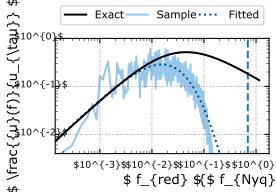
\includegraphics{PSD_Mesh_A_PNG.png}
    		\caption{%
    		    Diagramm direkt als .png importiert. Schriftarten und Schriftgröße werden nicht angepasst, mathematische Symbole können nicht verwendet werden.
    		}
    		\label{fig:png_import}
    	\end{subfigure}
    	\hspace{0.05\textwidth}
    	\begin{subfigure}[b]{0.45\textwidth}
    		\centering
    		\input{_B_mainmatter/images/PSD_Mesh_A.pdf_tex}
    		\caption{%
    		    Diagramm als .svg importiert. Schriftarten und Schriftgröße werden auf das Dokument angepasst und mathematische Symbole werden konvertiert.
    		}
    		\label{fig:svg_import}
    	\end{subfigure}
    \end{footnotesize}
\end{figure}

Es existieren mehrere Möglichkeiten die .svg-Grafiken einzubinden. Siehe \url{https://tex.stackexchange.com/questions/2099/how-to-include-svg-diagrams-in-latex} für eine detaillierte Beschreibung der folgenden beiden Methoden. 

\subsubsection{1) Einbindung als .svg}

Hierfür kann das Paket \href{https://www.ctan.org/tex-archive/graphics/svg}{svg} verwendet werden. Jede SVG-Datei, die mit dem Befehl \verb!\includesvg! übergeben wird, wird unter der Haube mit Hilfe einiger Zusatzprogramme konvertiert.

Leider funktioniert dies nicht immer problemlos, da die Zusatzprogramme meist nicht standardmäßig installiert sind. Ansonsten ist dies aber die zu bevorzugenden Variante.

Prinzipiell kann die \gls{SVG}-Grafik direkt wie folgt eingebunden werden:

\begin{Verbatim}
\begin{figure}
    \input{filename}
\end{figure}
\end{Verbatim}

\newpage

\subsubsection{2) Einbindung als .pdf\_tex}

Die \gls{SVG}-Grafiken müssen in Inkscape als .pdf und .pdf\_tex exportiert werden. Hierzu die \gls{SVG}-Grafik als .pdf speichern und die Option \flqq Text in PDF weglassen und \LaTeX Datei erstellen \frqq auswählen. Dadurch werden Alle Texte aus der .pdf entfernt, in die .pdf\_tex exportiert und werden beim Einbinden in das \LaTeX-Dokument mit den Dokumenteneinstellungen formatiert.

Dieser Schritt kann auch entweder durch die Erstellung eines Batch-Skriptes, dem direkten Export aus o.g. Programmen als .pdf\_tex oder der Programmierung eines Latex-Befehls welcher Inkscape nutzt um den .pdf\_tex Export durchzuführen automatisiert werden, siehe auch \url{https://github.com/BeneStrahm/pyLEK/tree/master/inkscape}.

Anschließend kann die Grafik wie folgt eingebunden werden:

\begin{Verbatim}
\begin{figure}
    \input{filename.pdf_tex}
\end{figure}
\end{Verbatim}

\newpage

\section{Diagramme und Grafiken mit tikz}
\label{subsec:tikz}

\subsubsection{Darstellung von Funktionen}

\begin{figure}[htb]
\centering
\begin{align*}
f(x)=\tanh(x)
\end{align*}
\begin{tikzpicture}
\begin{axis}
[
width=200pt,
height=200pt,
axis x line=middle, xmin=-4, xmax=4, xtick={-3,...,3}, xlabel=$x$,
axis y line=middle, ymin=-1.5, ymax=1.5, ytick={-1,...,1}, ylabel=$f(x)$,
scale only axis=true,
samples=101
]
\addplot[uniSdarkblue, mark=none, very thick]{tanh(x)};
%		\legend{$\tanh(x)$}
\end{axis}
\end{tikzpicture}
\caption[Tangens hyperbolicus Aktivierungsfunktion]{Tangens hyperbolicus}
\label{fig:05_AktivTan}
\end{figure}

\subsubsection{for-Schleifen bei der Grafikerzeugung}

\begin{figure}[htb]
	\centering
	\begin{tikzpicture}[]
	\tikzstyle{netnode}=[circle, inner sep=0pt, text width=22pt, align=center, line width=1.0pt]
	\tikzstyle{inputnode}=[netnode, fill=uniSlightgrey,draw=black]
	\tikzstyle{hiddennode}=[netnode, fill=uniSlightgrey,draw=black]
	\tikzstyle{outputnode}=[netnode, fill=uniSlightgrey,draw=black]
	\tikzstyle{signal}=[arrows={-latex},draw=uniSblack,line width=1pt,rounded corners=4pt]
	
	\def\nodedist{35pt}
	\def\layerdist{80pt}
	\def\pindist{20pt}
	
	\tikzstyle{every pin edge}=[signal]
	\tikzstyle{annot} = [text width=6em, text centered]
	
	\foreach \y in {1,...,3}
	\node[inputnode, pin={[pin edge={latex-}, pin distance=\pindist]left:Eingabe \y}] 
	(I\y) at (0,-\y*\nodedist) {$i_\y$};  
	
	\foreach \y in {1,...,4}
	\node[hiddennode] 
	(H1\y) at ($(\layerdist,-\y*\nodedist) +(0, 0.5*\nodedist)$) {$h_\y^1$};
	
	\foreach \y in {1,...,4}
	\node[hiddennode] 
	(H2\y) at ($(2*\layerdist,-\y*\nodedist) +(0, 0.5*\nodedist)$) {$h_\y^2$};
	
	\foreach \y in {1,...,2}
	\node[outputnode, pin={[pin edge={-latex}, pin distance=\pindist]right:Ausgabe \y}]
	(O\y) at ($(H21) + (\layerdist, -\y*\nodedist)$) {$o_\y$};
	
	\foreach \dest in {1,...,4}
	\foreach \source in {1,...,3}
	\draw[signal] (I\source) -- (H1\dest);
	
	\foreach \dest in {1,...,4}
	\foreach \source in {1,...,4}
	\draw[signal] (H1\source) -- (H2\dest);
	
	\foreach \dest in {1,...,2}
	\foreach \source in {1,...,4}
	\draw[signal] (H2\source) edge (O\dest);
	
	\node[annot, above=4pt of H11] (hl) {verborgene Schicht 1};
	\node[annot, above=4pt of H21] (hl) {verborgene Schicht 2};
	\node[annot] at (I1 |- hl) {Eingabe\-schicht};
	\node[annot] at (O1 |- hl) {Ausgabe\-schicht};
	\end{tikzpicture}
	\caption[Schematischer Aufbau eines künstlichen neuronalen Netzes] %hier kann ein alternativer/ verkürzter Text für das Abbildungsverzeichnis angegeben werden
	{Schematischer Aufbau eines künstlichen neuronalen Netzes \cite[Abb. nach][]{Frochte.2019}} %Bildunteschrift
	\label{fig:05_DNN}
\end{figure}

\newpage

\subsubsection{Einbeziehung von Daten aus CSV-Datei}

\setlength{\figureheight}{5cm}
\setlength{\figurewidth}{\textwidth}
\begin{figure}[htbp]
	\centering
	\begin{tikzpicture}
		\begin{axis}[
			width=\figurewidth,
			height=\figureheight,
			date coordinates in = x,
			xmin=2018-01-01 00:00,
			xmax=2018-01-08 00:00,
			minor x tick num=1,
			xtick={2018-01-01 12:00, 2018-01-02 12:00, 2018-01-03 12:00, 2018-01-04 12:00, 2018-01-05 12:00, 2018-01-06 12:00, 2018-01-07 12:00},
			set layers,cell picture=true,
			xticklabel={\day.\month},
			xlabel={2018},
			ymin=-0.1, ymax=1.1, ytick={0,0.5,1},
			no marks,
			scaled y ticks = false,
			ylabel={[\nicefrac{\%}{100}]}
			,]
			\addplot+[color=black ] table[x=Zeit, y=Shadestep, col sep=comma, skip first n=0] {_B_mainmatter/data/Example.csv};
			\legend{Shadestep};
		\end{axis}
	\end{tikzpicture}
	\caption[Photometrische Regelung der adaptiven Verglasung im Juli 2018, nach 500 Episoden]{Photometrische Regelung der adaptiven Verglasung nach 500 Episoden, für den Zeitraum vom 01. bis 07. Juli 2018} \label{fig:05_AVPhJun500}	
\end{figure}

\ifLuaTeX %PDFLaTeX kommt beim internen Speichermanagement schnell an seine grenzen, weshalb dieser Plot nur beim Kompilieren in LuaLaTeX angezeigt wird.
\subsubsection{Einbeziehung von Daten aus CSV-Datei und Gruppierung von Grafiken}

\begin{figure}[htb]
	\setlength{\figureheight}{5cm}
	\setlength{\figurewidth}{\textwidth}
	\centering
	\begin{tikzpicture}
		\begin{groupplot}[
			width=\figurewidth,
			height=\figureheight,
			date coordinates in = x,
			xmin=2018-01-01 00:00,
			xmax=2018-01-08 00:00,
			minor x tick num=1,
			xtick={2018-01-01 12:00, 2018-01-02 12:00, 2018-01-03 12:00, 2018-01-04 12:00, 2018-01-05 12:00, 2018-01-06 12:00, 2018-01-07 12:00},
			set layers,cell picture=true,
			xticklabel={\day.\month},
			xlabel={2018},
			no marks,
			scaled y ticks = false,
			group style = {group size = 1 by 7,
				horizontal sep =1cm,
				vertical sep = 0cm,},]
			
			\nextgroupplot[xlabel={},xticklabels={},ylabel={[°C]}]
			\addplot[color=black ] table[x=Zeit, y=T01, col sep=comma, skip first n=0] {_B_mainmatter/data/Example.csv};
			\legend{T01};
			
			\nextgroupplot[xlabel={},xticklabels={},ylabel={[klx]}]
			\addplot[color=black ] table[x=Zeit, y expr=\thisrow{B01}/1000, col sep=comma, skip first n=0] {_B_mainmatter/data/Example.csv};
			\legend{B01};
			
			\nextgroupplot[ylabel={[kW]}, ymin=-0.02, ymax=0.32, ytick={0,0.1,0.2,0.3},]
			\addplot+[color=black , name path=A] table[x=Zeit, y expr=\thisrow{QBeleuchtung}+\thisrow{QHeizung}+\thisrow{QKuehlung}, col sep=comma, skip first n=0] {_B_mainmatter/data/Example.csv};
			\addplot+[draw=none,name path=B, mark=none] table[x=Zeit, y expr=0, col sep=comma, skip first n=0] {_B_mainmatter/data/Example.csv}; 
			\addplot+[gray, fill opacity=0.1] fill between[of=A and B];
			\legend{Q\textsubscript{HEAT}+Q\textsubscript{COOL}+Q\textsubscript{LIGHT}};

		\end{groupplot}
	\end{tikzpicture}
	\caption[Kombinierte Regelung im Januar 2018, nach 500 Episoden]{Kombinierte Regelung nach 500 Episoden, für den Zeitraum vom 01. bis 07. Januar 2018} \label{fig:05_KomJan18}	
\end{figure}
\fi